\subsection*{Reference Element Map}


\begin{frame}[t]
%  \frametitle{Poisson Equation}
  \begin{block}{}
    \begin{itemize}    
  \item{
    The integrals are performed on a ``reference'' element $\alert<1>{\hat{\Omega}_e}$
    }
  \end{itemize}
  \end{block}
  %\vspace{-.3in}
  %\begin{center}   %Note: \centering is what makes the tables ``wiggle'' during slide transitions
  %% Three separate tabular elements.  The first column is an empty, fixed-width column designed
  %% to center the table without using centering commands.
    \only<1>
    {
    \begin{tabular}{p{.125\textwidth}ccc} \\
      &
      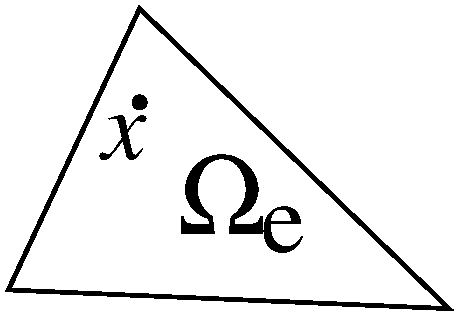
\includegraphics[width=.2\textwidth]{figures/physical_element}&
      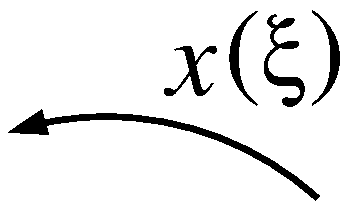
\includegraphics[width=.2\textwidth]{figures/map}&
      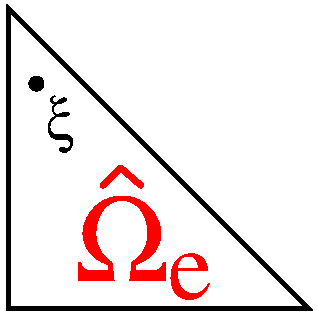
\includegraphics[width=.15\textwidth]{figures/reference_element_red}
    \end{tabular}
    }
    %
    \only<2>
    {
    \begin{tabular}{p{.125\textwidth}ccc} \\ 
      &
      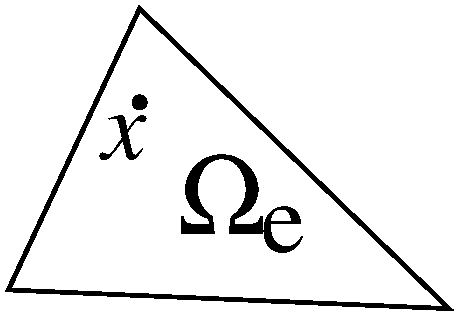
\includegraphics[width=.2\textwidth]{figures/physical_element}&
      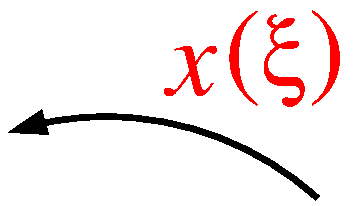
\includegraphics[width=.2\textwidth]{figures/map_red}&
      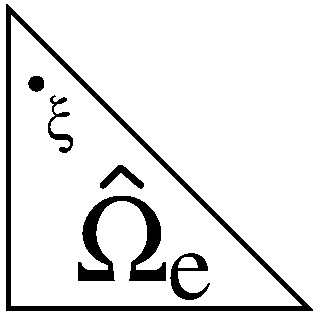
\includegraphics[width=.15\textwidth]{figures/reference_element}
    \end{tabular}
    }
    %
    \only<3>
    {
    \begin{tabular}{p{.125\textwidth}ccc} \\ 
      &
      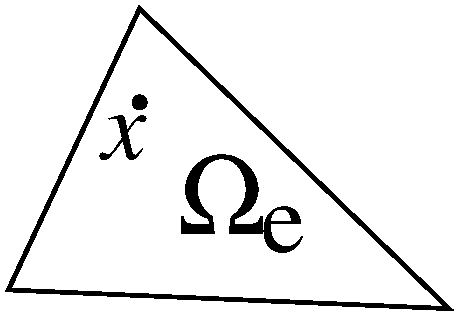
\includegraphics[width=.2\textwidth]{figures/physical_element}&
      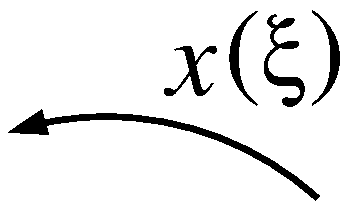
\includegraphics[width=.2\textwidth]{figures/map}&
      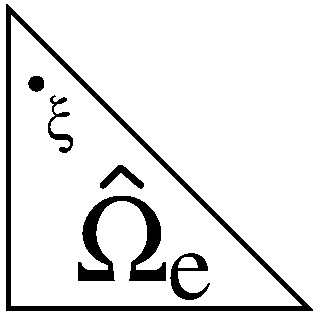
\includegraphics[width=.15\textwidth]{figures/reference_element}
    \end{tabular}
    }
    
%%     %% All in one table
%%     \begin{tabular}{ccc} \\ 
%%     %\fbox{
%%       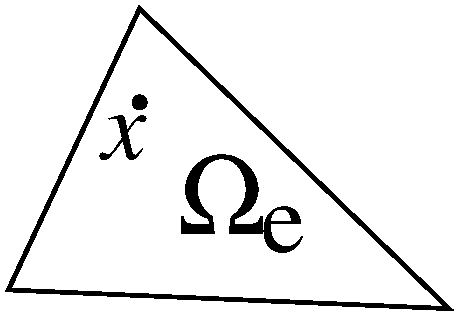
\includegraphics[width=.2\textwidth]{figures/physical_element}
%%     %}
%%        &
%%   \only<1,3->
%%   {
%%        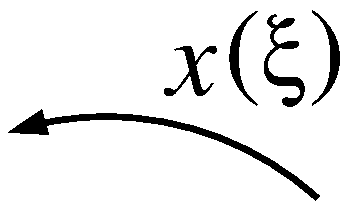
\includegraphics[width=.2\textwidth]{figures/map}
%%   }
%%   \only<2>
%%   {
%%        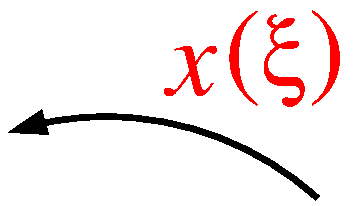
\includegraphics[width=.2\textwidth]{figures/map_red}
%%   }
%%        &
%%   \only<1>
%%   {
%%        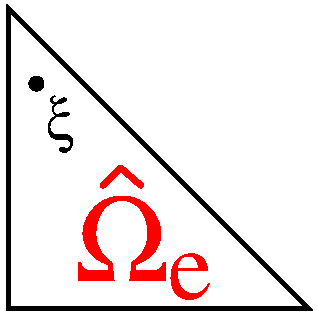
\includegraphics[width=.15\textwidth]{figures/reference_element_red}
%%        }
%%   \only<2->
%%   {
%%        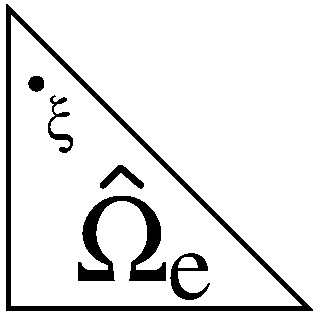
\includegraphics[width=.15\textwidth]{figures/reference_element}
%%        }
%%      \end{tabular}
  %\end{center}


  \only<2>
      {
	\begin{block}{}
	\begin{itemize}    
	\item{
	  The Jacobian of the map $\alert{x(\xi)}$ is $\alert{J}$.
	}
	\end{itemize}
	\end{block}
	\begin{equation}
	  \nonumber
	  \bv{F}^e_{i} = \int_{\Omega_e} f \phi_i dx
	  =  \int_{\alert{\hat{\Omega}_e}}
	  f (\alert{x(\xi)}) \phi_i \alert{|J|} d\alert{\xi}
	\end{equation}
      }

\only<3>
{
  \begin{block}{}
  \begin{itemize}    
  \item{
    %The gradients are transformed
    Chain rule: 
    $\nabla 
    = J^{-1}\nabla_{\!\xi}
    := \alert{\hat{\nabla}_{\!\xi}}$
  }
  \end{itemize}
  \end{block}
  \begin{equation}
    \nonumber
    \bv{K}^e_{ij} =
    \int_{\Omega_e}
    \nabla \phi_j \cdot \nabla \phi_i \;dx =
    \int_{\hat{\Omega}_e}
    \alert{\hat{\nabla}_{\!\xi}} \phi_j \cdot
    \alert{\hat{\nabla}_{\!\xi}} \phi_i \;|J| d\xi
  \end{equation}
}
\end{frame}
